\documentclass{beamer}
  \usepackage[utf8]{inputenc}
  \usetheme{Warsaw}
  \graphicspath{images/}
  \usepackage{amsmath} 
  \usepackage{amssymb}

  \title{Are New Technologies an issue for society?}
  \author{Clément CAUMES \& Mehdi MTALSI-MERIMI}
  \institute{UFR des Sciences Versailles - M1 Informatique}
  \date{Semestre 2} % RAJOUTER PLAN ICI

  \begin{document}

\section{Introduction}

  \begin{frame}
  \titlepage
  \end{frame}

\section{A curb for our planet}

\subsection{Destroy resources}

 \begin{frame}
\begin{block}{Issues of resources} 
	Increase of population, demands and productions induce :
	\begin{itemize}
		\setbeamertemplate{itemize item}[circle]
		\item Resource overexploitation
		\item Extinction of rare animals and plant species
	\end{itemize}
	\hspace{2.5cm}
	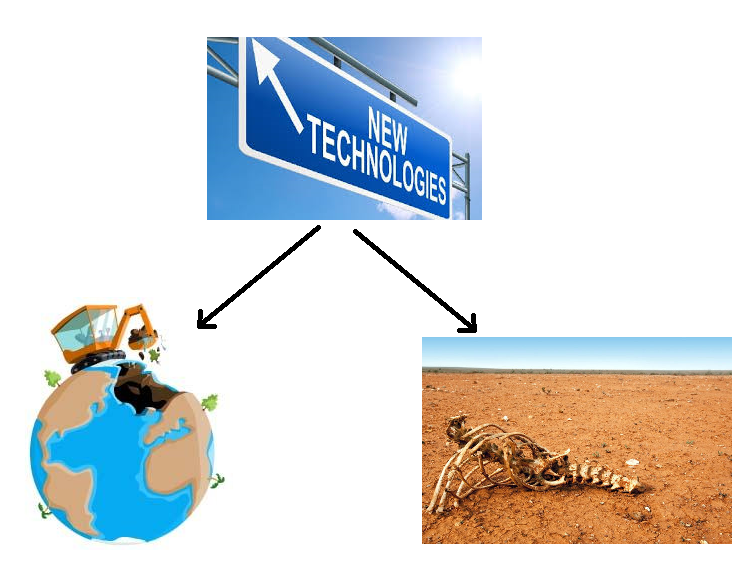
\includegraphics[scale=0.3]{pics/image1.png}
	\end{block}
\end{frame}

\begin{frame}

\begin{block}{Date of exhaustion of mineable resources} 
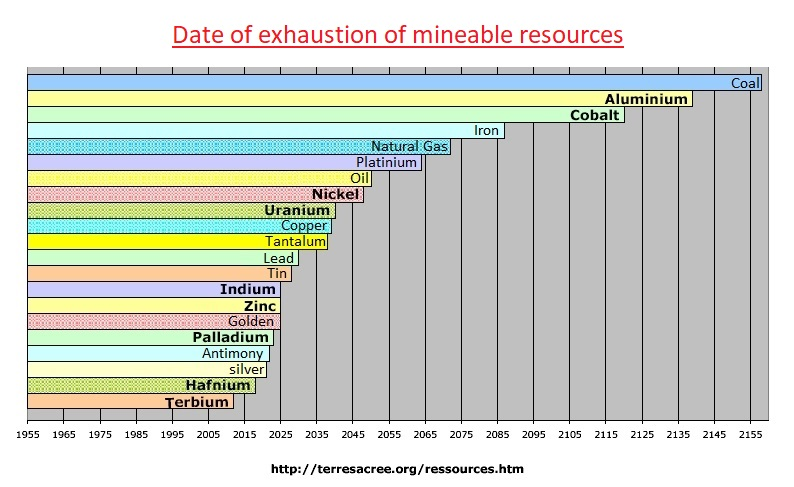
\includegraphics[scale=0.40]{pics/image2.jpg}
\end{block}

\end{frame}

\subsection{Contribute to the pollution}

 \begin{frame}
\begin{block}{Sustainable development = solution ?} 
	\begin{itemize}
		\setbeamertemplate{itemize item}[circle]
		\item Development of the economy
		\item Development of the social aspect
		\item Preservation of the environment
	\end{itemize}
	\hspace{2.5cm}
	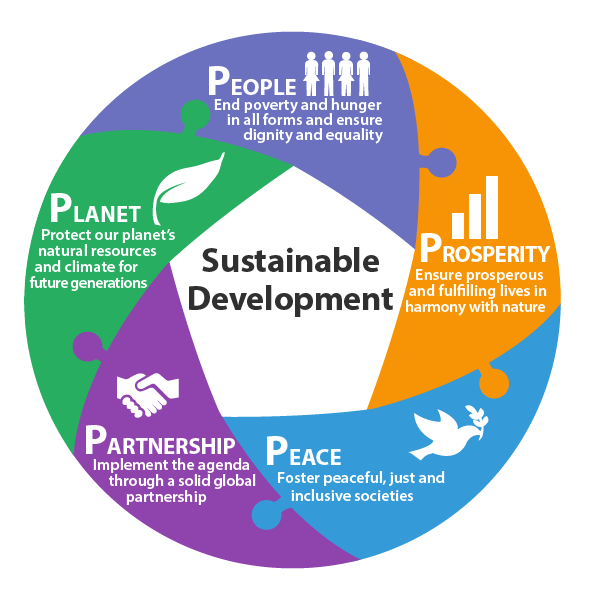
\includegraphics[scale=0.2]{pics/image3.png}
\end{block}
\end{frame}

 \begin{frame}
\begin{block}{Emissions of fossil carbon since 1800} 
	\hspace{4cm}
	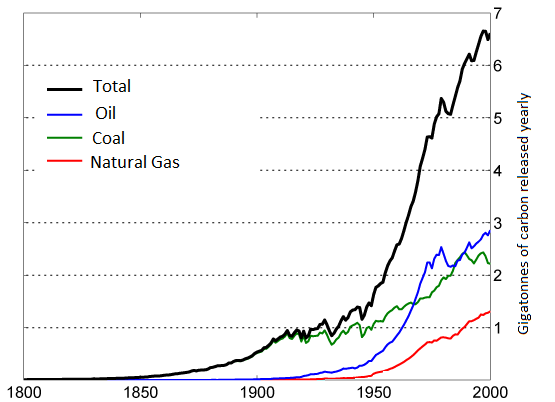
\includegraphics[scale=0.6]{pics/image5.png}
\end{block}
\end{frame}


\section{An impact for a social perspective}

\subsection{Increase addictions}

 \begin{frame}
\begin{block}{Addiction of new technologies} 
	\begin{itemize}
		\setbeamertemplate{itemize item}[circle]
		\item New technologies change the behaviour of young people
	\end{itemize}
	\hspace{4cm}
	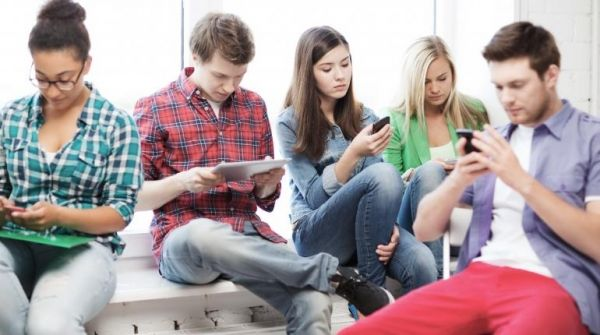
\includegraphics[scale=0.5]{pics/image6.jpg}
\end{block}
\end{frame}

\subsection{Creating Inequalities}

\subsection{Creating Conflicts}

\section{Conclusion}
      
\end{document}
